\documentclass{report}

\newcommand{\sign}{\begin{flushleft}
	\begin{tabular}{p{4in}@{}}
		\vspace{0.75cm}
		\hrulefill \\ \vspace{0.2cm}
		D\'ario Tavares Antunes, \today
\end{tabular}
\end{flushleft}}

\newcommand{\toolname}[1]{\emph{#1}}
\newcommand{\functionname}[1]{\texttt{#1}}
\newcommand{\malloc}[0]{\functionname{malloc}}
\newcommand{\free}[0]{\functionname{free}}

\newcommand{\todo}[1]{}

\usepackage[utf8]{inputenc}

\usepackage{hyperref}
\usepackage{xcolor}
\hypersetup{colorlinks,
	linkcolor={red!50!black},
	citecolor={blue!50!black},
	urlcolor={blue!80!black}
}

\usepackage[backend=biber,
style=alphabetic,
sorting=ynt]{biblatex}
\usepackage[nottoc,numbib]{tocbibind}
\addbibresource{references.bib}

\usepackage{graphicx}
\graphicspath{{img/}}

\usepackage{epigraph}

\begin{document}
	\hypersetup{pageanchor=false}
	\begin{titlepage}
	\begin{center}
		\vspace*{-2cm}
		
\includegraphics[width=\linewidth]{tcd}
		\vfill
		\textbf{\LARGE Eliminating Small, Transient Memory Allocations}\\
		\large
		\vspace{1.5cm}
		\textbf{D\'ario Tavares Antunes} \\
		B. A. (Mod.) Computer Science \\
		Final Year Project May 2018 \\
		Supervisor: Dr. David Abrahamson\\
		\vfill
		\Large
		School of Computer Science and Statistics \\
		O'Reilly Institute, Trinity College, Dublin 2, Ireland
	\end{center}
\end{titlepage}
	\hypersetup{pageanchor=true}

	\pagenumbering{roman}

	\section*{Declaration}
	I hereby declare that this project is entirely my own work and that it has not been submitted as an exercise for a degree at this or any other university.

\sign
	\pagebreak

	\section*{Permission To Lend}
	I agree that the Library and other agents of the College may lend or copy this report upon request.

\sign
	\pagebreak

	\section*{Abstract}
	Changes have been made to \toolname{cURL}, replacing short-lived dynamic memory allocations with stack allocations. Significant performance increases were claimed to result from these changes, and this project seeks to both validate those claims and make similar changes easier to perform in other codebases.

A plug-in was produced for the \toolname{Frama-C} static analysis platform, enabling it to detect small and short lived memory allocations in an intra-procedural scope.

Case studies were performed comparing the performance of code before and after the replacement of dynamic memory allocation with alternative allocation methods.

The impact of similar changes on the \toolname{cURL} codebase were analysed as a real world case study by comparing the performance of binaries built from it before and after the changes. 

An evaluation of the results of these case studies is then presented.

	\pagebreak

	\section*{Acknowledgements}
	I would like to thank my friends and family for consistently providing great support throughout the years. In particular, thanks are due to: my parents, for everything they have done to get me to this point; Tiago, for his endless support and thorough inflation of my ego throughout the years; Scarlett, for the myriad ways in which she's provided support and kept me in a healthy lifestyle.

I would also like to thank the various educators and academics who have led me to this goal. In particular I would like to thank David Abrahamson, my supervisor, for his help and guidance throughout this project.

Lastly, thanks are due to the general communities both online and not who nurtured my interests in Computer Science and in programming over the years.

	\pagebreak

	\tableofcontents
	\cleardoublepage
	\pagenumbering{arabic}

	\chapter{Introduction}
	\epigraph{640K ought to be enough for anybody.}{Not Bill Gates}

Despite the often misattributed epigraph above often being used to mock past beliefs that some amount of memory should be enough for any reasonable purposes, the mentality behind it is still pervasive.

With the broad availability of large amounts of computational power, memory and storage, conservation or efficient use of the same is often overlooked in programming. This is largely perpetuated by the (often valid) view that programmer time is more valuable than the benefits that more efficient but more complex code brings.

However, there remain situations where these benefits are in fact worth the effort required. One of these such cases is in code intended to be deployed in embedded or mobile devices, where resources are limited and preservation of power is essential. \\
A blog post \cite{curlmalloc} by Daniel Stenberg, original author of the \toolname{curl} command line tool and ubiquitous URL data transfer tool, is a retrospective on an attempt to reduce unnecessary heap allocations.

Inspired by that post, the aim of this project is to produce a tool to identify cases where similar changes could be made in order to potentially reduce a program's energy and processing power footprint, and at the same time improve its performance.

\section{Report Structure}

The report is structured as follows:

\begin{itemize}
	\item{Chapter 2 provides background on the project, including further information on the changes to \toolname{cURL} that inspired this project, as well as laying out the objectives of the project}
	\item{Chapter 3 describes the goals of the plugin developed, the platform it built upon, difficulties encountered in development, and the final state of the plugin}
	\item{Chapter 4 covers three case studies, two written intentionally to trigger certain behaviours to maximise the optimisation's effect, and one which simply involves isolating Stenberg's changes and testing their impact}
	\item{Chapter 5 examines the results and outcomes of the case studies and state of the plugin, as well as including a short discussion on potential benefits of future work in this area}
	\item{Chapter 6 describes the state of the art in related areas to the project}
	\item{Chapter 7 describes some areas with potential for future work}
\end{itemize}


	\chapter{Background and Objectives}
	This chapter will describe the changes made to \toolname{cURL} and discuss what situations lead to the production of code which needs this change applied to it. The project goals are then defined in the context of the pattern to be detected and benchmarked.

\section{Background on the Changes}\label{backgroundsec}

\toolname{cURL}'s first dated change was introduced in April of 1998~\cite{curlrelease}, with three versions already having been released before that. When introduced, guidelines for contributors were loose and didn't particularly discourage varying programming styles or encourage adherence to existing styles in the codebase~\cite{curlcontribute1999}. In the 20 year interim, stricter guidelines have been introduced; all changes require tests, must be sufficiently atomic, must include documentation, and so on~\cite{curlcontribute2017}.\\
However, over 150,000 lines of C have been added in that period of time and under potentially weaker requirements. As a result, there are plenty of places where improvements can be made.

Stenberg's post discusses two allocation related changes~\cite{curlmalloc}. The first involves rewriting some generic linked list functions to avoid all dynamic memory allocation, while the second involves rewriting a polling function to reduce the number of dynamic memory allocations performed.

\subsection{Linked List Changes}

The change involved rewriting data structs that can be inserted into linked lists as follows:

\lstinputlisting[style=CStyle]{samples/llistchanges.c}

In order to insert the \varname{data\_before} struct into a linked list, a \varname{llist\_node} struct would have to be allocated separately and its data member set to a pointer to the \varname{data\_before} struct. Removing the \varname{data\_before} struct from the linked list would then require \free{}ing the \varname{llist\_node}.\\
Doing the same with the \varname{data\_after} struct would require no extra allocations/deallocations or pointer assignments as the data member of its embedded \varname{llist\_node} would only need to be set once.

This has two beneficial results:

\begin{itemize}
	\itemsep-0.25em
	\item Linked list functions can't fail due to memory constraints any more, simplifying logic that uses them
	\item One less \malloc{} and \free{} per linked list operation
\end{itemize}

According to Stenberg in his blog post, these changes led to a modest reduction in the number of allocations in a simple benchmark (from 115 allocations to 80, or a 26\% reduction)~\cite{curlmalloc}. He also notes that these changes are effectively free and improve the code quality.

\subsection{Polling Function Changes}

The polling function in question is \functionname{curl\_multi\_wait}. The function takes as input a list of file descriptors\footnote{A file descriptor is part of the POSIX API, providing a uniform interface to similar but distinct interfaces such as files, hardware devices, network sockets and so on. \toolname{cURL} further abstracts the concept for added portability. The specifics are not important here.}, polls each one and returns with an error code (indicating whether the descriptors were polled successfully or if there was some issue).\\
For the purposes of polling, \toolname{cURL}'s internal abstraction is accepted alongside regular file descriptors. These are all copied to a dynamically allocated block of memory to make polling from the two distinct sources simpler.

The expectation is that \functionname{curl\_multi\_wait} will be used in conjunction with other functions for bulk operations on sets of file descriptors in a polling loop. Due to internal constraints on timeouts, this means that \functionname{curl\_multi\_wait} could be called as often as 1000 times per second, each time potentially calling \malloc{} to produce the block of memory. Removing this \malloc{} should lead to a significant reduction in the number of allocations performed overall.

The change made here was simple, and the one of interest for this project. In the common case (as claimed by Stenberg without mentioning how its commonness was determined), \functionname{curl\_multi\_wait} was changed to avoid the \malloc{}, instead using a stack allocated block of memory when few file descriptors were passed to it.\\
Stenberg claims that in a simple benchmark this change resulted in a 99.62\% decrease (33,961 to 129) in the number of \malloc{} calls.

\subsection{Results of the Changes}

The version of the tool built with these changes was then compared in a fully local benchmark (to avoid any impact of network connectivity or other external factors) to the previous release. Stenberg reports that it performed 30\% faster, transferring 2900~MB/sec vs the previous version's 2200~MB/sec.

However, this comparison attributes all performance and allocation differences to these two commits, despite there having been 231 commits in total between the two versions. Stenberg highlights this, but adds a caveat that none of them spring to mind as having an impact on the number of allocations or significant performance changes.

\section{Objectives of this Project}

The project has two main objectives, in which \textit{patch} refers to applying changes which replace dynamic allocation with stack or static allocation.

\begin{enumerate}
	\itemsep-0.25em
	\item Produce a tool that can detect sites where there is potential to perform the patch
	\item Determine the impact that the patch can have on performance
\end{enumerate}

\subsection{Tool to Detect Potential Patch Sites}

The general pattern of sites where a patch can be applied appears similar to the code listing below

\lstinputlisting[style=CStyle,label=patternsample]{samples/pattern.c}

where the \malloc{} and \free{} on lines 2 and 4 could instead be replaced with stack allocation\footnote{The details of how stack allocation would be achieved in this situation are explored further later, but are unimportant at this point}, avoiding both of those calls and indeed completely avoiding any risk of a memory leak\footnote{A memory leak refers to the loss of a pointer to a dynamically allocated block of memory (using the \malloc{} family or similar) before it is \free{}d, resulting in the memory being consumed but useless until the program exits}.

The concept is simple: some amount of memory is allocated, used for a short amount of time, then \free{}d. In a small example, the pattern is obvious and easy to detect, or even to not introduce in the first place. However, as seen in the real world \toolname{cURL} example in the blog post, these patterns are introduced, either by mistake or for simplicity (relative to more complex code required for safe stack allocation).

There are also further considerations to be taken before replacing a heap allocation with a stack allocation, and even more considerations if it's to be replaced with static allocation. A non-comprehensive list follows, where some items result in undefined behaviour\footnote{Undefined behaviour in C is the result of any operation which has no defined semantics, and its outcome may vary from implementation to implementation or even run to run. To the compiler, UB is equivalent to $\bot$, and so it may generate any code if it can detect UB} (UB)

\begin{itemize}
	\itemsep-0.25em
	\item Stack overflow can be caused by stack allocation of a large amount of data, resulting in UB
	\item A pointer to the data escaping its scope would result in a dangling pointer, whose dereferencing results in UB
	\item The variable may be assigned to at various different points, complicating stack allocation (depending on the method used)
	\item If static allocation is used, it must be guaranteed that the function can only be executed in one site at a time to avoid multiple sites overwriting each other's data, and the function will not be reentrant\footnote{Reentrancy is a property of a function that may be entered while a previous invocation is still executing without affecting the correctness of either execution, and is a required property of recursive functions}
\end{itemize}

The tool should take as many of these cases into consideration as possible, to avoid suggesting applying the patch at sites where it would cause errors.

Development of the tool is discussed in depth in Chapter~\ref{implementation}.

\subsection{Determining the Patch's Impact on Performance}

First, the maximum expected performance impact should be found, to set an expectation of what the best case result would be. To that end, two bespoke benchmarks were written: one to attempt to trigger certain slow behaviours in the allocator that can then be avoided by stack allocating instead; another to simulate a simple but realistic benchmark to test the results of the patch in isolation.

Next, in order to determine the performance change in a real world situation, the \toolname{cURL} changes were tested in complete isolation from other commits to determine how much of the performance difference was a result of the allocation changes.

The benchmarks are discussed in depth in Chapter~\ref{studies}.


	\chapter{Implementation}
	Two initial approaches to create the tool were considered: hooking directly into the compiler to detect the pattern and automatically patch it (when enabled, and when the pattern is detected with sufficiently high confidence); or creating a plug-in for an existing static analysis platform which could be manually run on existing codebases to detect the pattern. A decision was made, largely for reasons of pragmatism and convenience, to follow the second approach.

In particular, the time to become familiarised with the extensive and complex codebase of a production compiler (which may not evene provide sophisticated value analysis) would lead to a highly reduced chance that the project would be complete within the time allowed.

\section{Goals of the Plug-in}

There were a small set of goals for the plug-in to achieve, both functional and non-functional.

\subsection{Non-Functional Goals}

The non-functional goals are as follows:

\begin{itemize}
	\item There should be little to no modification of any existing code required to use the plug-in to a satisfactory degree
	\item There should be a minimal amount of false positives wherein the plug-in suggests a site where the patch cannot be applied
	\item Interaction with the plug-in should match the normal mode of interaction for the platform it builds on
\end{itemize}

These goals should ensure that the barrier to entry to using the plug-in is as low as possible, as it can be used directly on existing code, even if the static analysis platform itself has never been used on that code. Additionally, avoiding false positives makes it more likely that action will be taken on the plug-in's results by minimising the amount of data users have to trawl through~\cite{infervideo}. Lastly, ensuring all interaction with the plug-in matches what's expected of its platform makes its adoption in systems already using the static analysis platform even easier.

\subsection{Functional Goals}

The functional goals are as follows:

\begin{itemize}
	\item When a site where the patch can be applied is found, the user should be notified
	\item Where possible, a diff patch\footnote{A diff patch is an encoding of a set of changes that can be automatically applied with a standard tool to a file to effect a change} should be produced to apply the patch easily
\end{itemize}

Notifying the user is a fairly self-explanatory goal, as there's no point detecting an issue and not noting it. The exact form of the notification isn't important, but should provide as much information as possible without overwhelming the user, allowing them to make a reasonable decision about what action to take.

The diff patch is more complicated, but would be incredibly useful. If the plug-in's could guarantee that a certain site could be patched safely before producing a diff patch, it could be added into a pre-compilation step to rewrite the pattern silently. This would allow the source code that users work on to remain simple and as they wrote it while gaining any performance benefit from the patch.

\section{Static Analysis Platform}

There are a number of static analysis tools built for C over the years, of which a small number were chosen based on apparent activity of their development and popularity (as a proxy for likelihood to be well supported and modern). The short-list which the eventual target platform was chosen from consisted of \toolname{clang-analyzer}~\cite{clang-analyzer}, \toolname{Frama-C}~\cite{frama}, and \toolname{Infer}~\cite{fbinfer}.

\toolname{clang-analyze} is written in C++, matching the \toolname{clang} codebase in originates from and resides in. \toolname{Frama-C} and \toolname{Infer} are both written in OCaml, though while \toolname{Frama-C} builds up its own AST\footnote{An Abstract Syntax Tree (AST) is a tree-based representation of a program, with each node representing a construct appearing in the source code}, \toolname{Infer} hooks into \toolname{clang-analyzer}.

The tools that were not chosen are discussed in further depth in Chapter~\ref{state_of_the_art} in comparison to \toolname{Frama-C} in a retrospective manner.

\section{The \toolname{Frama-C} Platform}

The static analysis platform chosen was \toolname{Frama-C}. \toolname{Frama-C} has an emphasis on on correctness, providing its own language for functional specifications which can be provided alongside the code. While this is of no particular interest to this project thanks to the first functional goal, it assists in reducing false positives thanks to its conservative approach and care around sites of potential undefined behaviour~\cite{framauser}. Additionally, that specification language is used by the platform to provide properties of standard library functions such as \malloc{} and \free{}, which is essential to the project's analysis.

However, and of more interest to the project, it also has a plug-in architecture, which makes it easy to extend and build on. In particular, it enables plug-ins to interact, which allows new plug-ins to use functionality exposed by existing plug-ins thereby reducing the workload required within the plug-in itself. This was the primary factor in the choice of \toolname{Frama-C} over the other two platforms~\cite{framaarch}.

\subsection{Source Code Processing}

\toolname{Frama-C} produces an AST which plug-ins can then operate on. The version of the code exposed to plug-ins is normalised by Frama-C, which prevents duplication of efforts in handling unusual edge cases enabled by C's permissive design. As an example, consider the following C functions (which are intentionally contrived)

\lstinputlisting[style=CStyle]{samples/contrived.c}

This is normalised into something like the following by \toolname{Frama-C}

\lstinputlisting[style=CStyle]{samples/normalised.c}

We note in particular that rewrites are performed in order to avoid multiple operations occurring on a single line, such as splitting out the evaluation of return values and their actual return, or the evaluation of expressions involving function calls and the actual function call. This prevents an arbitrarily complex AST from being constructed.

The AST itself as provided to plug-ins to traverse is also annotated. It can be annotated in the source code itself, using \toolname{Frama-C}'s ACSL\footnote{ANSI/ISO C Specification Language, used to formally define function contracts} to add specifications~\cite{framaacsl}, or annotations can be added by other plug-ins as they discover properties of the code~\cite{framaplug}.

The root of the AST is a representation of the file being processed, which contains a collection of globals, of which we're only interested in functions. Other globals include declarations of variables, types, structs, unions, enums, and some other miscellaneous things.

Within a function node we're interested in its statement list, which contains statements of various kinds, such as a plain instruction with no control flow, which can include a variable declaration and assignment, or a reassignment of an existing variable. These are the exact subsets of statements in which a \malloc{} can occur after normalisation of the AST, including the unusual case of a \malloc{} that's not assigned to anything.

\toolname{Frama-C} alone doesn't provide any sort of value or escape analysis, instead leaving this to be provided by plug-ins. The primary plug-in providing these features is called \toolname{Evolved Value Analysis} (\toolname{EVA}). Note that this distinction is largely symbolic, as \toolname{EVA} is statically connected to the \toolname{Frama-C} kernel, unlike regular plug-ins.

\subsection{The \toolname{Evolved Value Analysis} Plug-in} \label{EVA}

\toolname{EVA} provides, at any given point in the AST, a set or interval describing values possible at a given point. Values can be requested for expressions or variables with respect to a given statement, and they can be evaluated either before or after execution of that statement. \toolname{EVA} also performs semantic constant folding, allowing it to be used even on code including loops~\cite{framaeva}.

Values can be described as a discrete set of values, as an interval, or as an interval skipping regular values. When \toolname{EVA} determines that one of the representations is becoming too large, it can degenerate the value to a broader description that contains all of the original values. As an example, take the following:

\lstinputlisting[style=CStyle,firstline=21,lastline=38]{samples/eva.c}

Assuming that the level of semantic constant folding \toolname{Frama-C} is permitted to do is high enough to fully evaluate the loop and that \varname{NUM\_PRIMES} is set to 8, \toolname{EVA} produces the following values at the end of the loop

\begin{table}
	\centering
	\begin{tabular}{lc|lc}
		\toprule
		\textbf{Variable} & \textbf{Values} & \textbf{Variable} & \textbf{Values} \\
		\midrule
		\varname{morePrimes[0]} & \{2\} & \varname{morePrimes[4]} & \{11\} \\
		\varname{morePrimes[1]} & \{3\} & \varname{morePrimes[5]} & \{13\} \\
		\varname{morePrimes[2]} & \{5\} & \varname{morePrimes[6]} & \{17\} \\
		\varname{morePrimes[3]} & \{7\} & \varname{morePrimes[7]} & \{19\} \\
		\varname{randVal} & [0..32767] & \varname{index} & \{8\} \\
		\varname{randPrime} & \{2; 3; 5; 7; 11; 13; 17; 19\} & & \\
		\bottomrule
	\end{tabular}
\end{table}

In particular, note that each item in the array \varname{morePrimes} is tracked separately by \toolname{EVA}, that \varname{randPrime} can take on any of the prime values, that \varname{randVal} can take on any values between 0 and \toolname{Frama-C}'s \varname{RAND\_MAX}, and that variables that can only take on a single value are considered to have a value which is a singleton set.

Next, we consider the values reported if the semantic constant folding allowed is set too low to evaluate anything past the first prime. The values reported are now

\begin{table}[h]
	\centering
	\begin{tabularx}{\linewidth}{>{\hsize=1.1\hsize}X >{\hsize=1.3\hsize}X | >{\hsize=0.6\hsize}X >{\hsize=1\hsize}X}
		\toprule
		\textbf{Variable} & \textbf{Values} & \textbf{Variable} & \textbf{Values} \\
		\midrule
		\varname{morePrimes[0]} & \{2\} & \varname{index} & \{8\} \\
		\varname{morePrimes[1..7]} & [3..2147483647] or UNINITIALIZED & \varname{randVal} & [0..32767] \\
		\varname{randPrime} & [2..2147483647] & & \\
		\bottomrule
	\end{tabularx}
\end{table}

This time we note that EVA can no longer determine whether the loop ever terminates and cannot determine the values for all indices of the \varname{morePrimes} array, nor if they're ever initialised (due to the possibility of overflow in \varname{current} without index being incremented sufficient times to exit the loop). As expected, \varname{randPrime}'s possible values also cannot be determined, as it depends on full evaluation of all values in \varname{morePrimes}. However, the other variables do not depend on the loop, so they can be correctly evaluated regardless.

Next, increasing \varname{NUM\_PRIMES} to 9 causes \toolname{EVA} to decide \varname{randPrime} has too many values, so it reduces its precision to [2..23] which still contains all the correct values with as much precision as possible without storing the individual values.

Additionally, changing line 12 so that \varname{randPrime} is assigned \varname{current * 4} causes \toolname{EVA} to again degenerate its set of values into [2..76]0\%2, which is the most complicated value type \toolname{EVA} can produce, and indicates that values start at 2 with an offset of 0 and every second value is potentially valid. This includes all the valid values (\{8; 12; 20; 28; 44; 52; 68; 76\}), but is less precise than an alternative interval of [8..76]0\%4. It's not clear why \toolname{EVA} choose one instead of the other.

While this covers all simple values such as integers, floats, and even structs (which function similar to an array, where each member is separately displayed), it doesn't cover pointers. There are two kinds of pointer which are represented identically. The first is a pointer to an existing variable such as \varname{\&randPrime}, while the second is a pointer created by a call to a function like \malloc{}. Both types are represented as \varname{\{\{ \&varname \}\}}, where \varname{varname} is either the name of the variable pointed to, or something of the form \varname{\{\{\&\_\_malloc\_main\_l33 \}\}} in the case of \malloc{}, where a unique variable name is generated, representing a point in heap memory which \toolname{EVA} calls a Base.

Bases can be collected in sets, same as regular values, but cannot form an interval. There is also a special pointer, \varname{NULL}, representing exactly that and marked as a potential return value by \toolname{Frama-C}'s internal version of \malloc{}, although that can be disabled by one of \toolname{EVA}'s options~\cite{framamalloc}. Clearly, bases are of particular interest for the project.

\section{Development of the \toolname{Forgetful} Plug-in}

A plug-in development guide is provided to aid new developers in the \toolname{Frama-C} environment to create their own plug-ins~\cite{framaplug}. The guide outlines some common use-cases, providing some code samples and best practices. Parts of these are used together to create the \toolname{Forgetful} plug-in.

\subsection{Visitor Pattern}

For any plug-in that doesn't require direct access to the AST for any particular reason, the development guide recommends usage of one of the provided visitor classes built-in to \toolname{Frama-C}.

The visitor classes are classes implementing the visitor design pattern, intended for usage by developers who can extend and override only the specific methods they're interested in. The design pattern itself is described as

\begin{quote}
	Represent an operation to be performed on the elements of an object structure. Visitor lets you define a new operation without changing the classes of the elements on which it operates.~\cite{gof}
\end{quote}

The benefit of this pattern is that it allows the easy addition of new operations on the AST, with the downside being that it's difficult to add new types of node to the AST, but given the nature of the AST new types of nodes are rare.

Concretely, for the development of the plug-in, this means that it can simply extend the in-place visitor (since the plug-in will not modify the AST itself, otherwise it would have to use the copy visitor to avoid corrupting information already attached to the AST~\cite{framaplug}) and override the functions for visiting individual statements and for visiting the function declaration node. \\
This will allow the plug-in to track which function it's currently in for scoping purposes, and to inspect the contents of statements in order to determine if they contain a \malloc{} or \free{}.

\toolname{Frama-C}'s documentation is limited, with many types having no documentation or referring the reader to either the plug-in development guide or the user guide with no indication of what section within the guides are relevant. As such, determining what purpose certain nodes in the AST served had to be determined through trial and error. For example, the \texttt{Block} node represents a block (such as a loop body) and as such contains a list of statements, but the visitor doesn't have to traverse those statements as they're actually duplicated.\\
Trial and error was also the method used to determine which nodes \malloc{} and \free{} could appear in after normalisation of the AST.

\subsection{Allocation Tracking}

Allocation tracking occurs only within any given function so as to ensure any allocations whose free site is found are short-lived, and specifically inter-procedural. This is non-essential, but is the easiest case of the pattern to replace with stack allocation.

To actually track allocations, a hashtable mapping a base's unique ID to the site where it was allocated is created. Each time a new function is visited, the hashtable is cleared to prevent previously seen allocations in different functions from being erroneously reported when they're \free{}d elsewhere.\\
The unique base ID is provided by \toolname{Frama-C}, and doesn't change throughout the analysis, making it ideal to look up bases when they are \free{}d to determine if they're short-lived.

Only allocations of a configurable maximum size or less are added to the hashtable to ensure that the only ones reported are those that can feasibly be stack allocated instead. Their location (filename and line number) is stored along with the statement they originated in so that the notification to the user can clearly indicate where changes are to be made.\\
For example, in the code listing in Section~\ref{patternsample}, the following is reported by \toolname{Forgetful} if it can determine that \varname{alloc\_size} is small enough to report.

\lstinputlisting[breaklines=true]{samples/forgetful_output.txt}

On a \free{}, \toolname{EVA} is used to determine what bases it could be freeing, and from there its ID is used to determine if the base identifies a small allocation and where it was allocated using the aforementioned hashtable.

Of course, not all allocations have a size that can be statically determined, with many instead having an interval as described in Section~\ref{EVA}. In order to simplify application of the patch in cases where the allocation size is an interval, these are only reported if the maximum value of the interval is less than or equal to the configured maximum size to report. However, this means that the plug-in cannot detect the case described by Stenberg in \toolname{cURL}~\cite{curlmalloc}, as the allocation was not always below the size chosen for stack allocation.\\
Different behaviour for intervals could be added, to allow for cases where stack allocation or heap allocation are decided between at run-time.

It's also worth noting that bases are independent of the variable names they're allocated to. Take the following section, where \varname{TOO\_LARGE} and \varname{SMALL\_ENOUGH} are appropriately defined so as to ensure the plug-in doesn't and does report the allocations respectively.

\lstinputlisting[style=CStyle]{samples/allocbranching.c}

The plug-in will report the allocation on line 3 even though \varname{val} can also be too large to report. This is because \varname{val}'s value is found by \toolname{EVA} to be a set of bases (from lines 1 and 3) where one is too large to report and the other is small enough, rather than describing it as a single base with a range which extends enough as to be too large.

This differs from the following example, in which there is only one base which has an interval too large to report as its size.

\lstinputlisting[style=CStyle]{samples/valbranching.c}

\subsection{Difficulties Encountered}

A number of difficulties were encountered throughout the project, described below.

\subsubsection{Build and Installation}

An initial and unexpected difficulty was the installation of \toolname{Frama-C} itself. A bug in one of its dependencies resulted in it being unable to compile, which made it impossible to install from source with no binaries available. A few patches (which all had to be applied together) for the issue were found online, not yet applied to the dependency despite having been available and known to the maintainer for a few months. To enable \toolname{Frama-C} to be built, the patches were applied during the build process.

This is more complicated than it sounds, as the build process downloaded new sources which needed to be patched as well, requiring a total of 3 or 4 patches which must be applied only once to any given file and before the next part of the build process started using those files. A script was eventually written to patch files on the fly once they were created, and run alongside the build process.

\subsubsection{OCaml and \toolname{Frama-C} Learning Curve}

As expected, there was a significant learning curve involved in learning both a new language, OCaml, and a new platform, \toolname{Frama-C}. Thanks to OCaml's similarity to languages such as Java and Haskell, some of this learning curve was mitigated due to familiarity with those languages. Having no prior experience developing part of or even using a static analysis tool, \toolname{Frama-C} was still difficult but manageable to broach thanks to both the user manual~\cite{framauser} and the plug-in development guide~\cite{framaplug}.

\subsubsection{Kernel and Core Plug-in Documentation}

Despite \toolname{Frama-C}'s lengthy guides for both users and plug-in developers, its documentation suffers from a lack of structure and detail. The plug-in development guide walks the developer through the development of a basic hello world style plug-in, building up to the currently recommended plug-in architecture. Once the basic structure is attained, the guide branches into a handful of sample plug-ins, jumping between \toolname{Frama-C}'s capabilities in a somewhat incoherent manner. By this point enough information has been provided to start on development however, so the API documentation provided separately is generally sufficient.

One case in which the API documentation proved insufficient was in its description of bases. In particular, functions are provided that allow translation from a base to variable info, which initially seemed to provide a simple way to perform most of the analysis. A base could simply be retrieved at the \free{} site, and have variable info retrieved from it to determine its allocation site and size. However, while variable info should include its allocation site, the variable info produced from a base doesn't include valid location data. This is why allocations have to be tracked forwards from the \malloc{} instead.

\toolname{EVA}'s documentation was the most lacking, with the majority of its manual being dedicated to users interacting with \toolname{EVA} through ACSL or the \toolname{Frama-C} GUI\@. In the entire manual, there is only one mention of an \toolname{EVA} API, which is the \functionname{value} function. However, the \functionname{value} function only returns the value before a statement has been executed and the Forgetful plugin needs access to the result after a \malloc{} call. A solution was eventually found online~\cite{foldstate}, but searching for one led to significant delays.

\section{Final State of the Plug-in}

The state of the Forgetful plugin is most easily communicated by examining results from running the analysis on various code samples.

\lstinputlisting[style=CStyle]{samples/recurse.c}

The above code listing produces no output from \toolname{Forgetful}, and the output from \toolname{EVA} indicates that the issue is with the function \functionname{recurse\_and\_free}. In particular, \toolname{EVA} can't determine whether the function terminates as it doesn't currently support recursion. Since \toolname{Forgetful} depends on \toolname{EVA}, it also can't analyse recursive functions.

The following code listing describes inline which allocations are reported as replaceable with stack allocation. The default max allocation size to report on was set to 48 bytes, based on the results discussed in Chapter~\ref{studies}.

\lstinputlisting[style=CStyle]{samples/demo.c}



	\chapter{Case Studies}
	This chapter will include, for each case study: reasoning under which that particular case study was chosen; predictions of the results; the code for the benchmark, or a reference to where the code can be found; results of the benchmark; and a discussion of the results compared to the conclusion.

For the code used in the benchmarks, refer to Appendix~\ref{codeappend}.

\section{Specialised Benchmark, Sorting}

The first benchmark involves minimal allocations and a large amount of busy work.

The benchmark setup code creates input data of an array of structs containing a random value and a sequential ID (which isn't used). It then calls each of the four benchmarking functions described below a large number of times (10,000 to 20,000 times) in a row each, timing how long each execution takes in total.

The benchmarking functions each perform a single allocation before copying the input buffer into the newly allocated block. How this allocation is performed is the core difference. The four types of allocation used are described in Table~\ref{alloctype}.

Note that \functionname{alloca}\footnote{\functionname{alloca} performs a stack allocation at runtime in a similar manner to \malloc{}, but does not perform checks for whether the stack will overflow as a result and doesn't require \free{}ing as restoring the stack pointer will automatically free the block} is used despite its unsuitability for safe and portable code. This is to simplify ensuring that there is always enough space in the \functionname{stack} benchmark function, in which errors are not fatal.\\
Another caveat to the use of \functionname{alloca} is that while it appears to be a standard library function, it's not actually part of the ANSI/ISO-C standard~\cite{c11std} and is simply replaced inline by compiler implementations. This causes portability concerns.

\begin{table}
	\centering
	\begin{tabularx}{\linewidth}{>{\hsize=0.6\hsize}X >{\hsize=1.4\hsize}X}
		\toprule
		\textbf{Allocation Type} & \textbf{Description} \\
		\midrule
		\functionname{malloc} & Performs the allocation with \malloc{}, providing a base performance to compare against. \free{}s the allocated block before returning \\
		\functionname{stack} & Performs the allocation with \functionname{alloca} regardless of the size of the input data even though this would introduce a significant risk of stack overflow in real code. No \free{} required \\
		\functionname{dynamic} & Performs the allocation with \malloc{} if the input data is larger than a given threshold (in this case, 64 items), otherwise uses an array of static size declared as a local variable (and, hence, stack allocated as part of the calling code). \free{}s before returning if required \\
		\functionname{external} & Performs no allocation, instead taking a parameter of a sufficiently large buffer to copy data to, which it doesn't \free{}. Acts as a control as no allocation is performed and so it should be the fastest \\
		\bottomrule
	\end{tabularx}
	\caption{Allocation Types}\label{alloctype}
\end{table}

\subsection{Program Reasoning}

This benchmark was chosen to provide a sort of floor for performance changes due to application of the patch, as a minimal amount of time should be spent in allocations to be gained back by more efficient allocations.

\subsection{Predictions}

It is expected that the \functionname{external} allocation method should be fastest, as it spends no time performing allocations. \\
The \functionname{stack} allocation method should be the next fastest, not requiring a \free{} or finding of a suitable block by \malloc{}, and should maintain a small performance increase even for larger input sizes, although this will be dwarfed by the time spent sorting. \\
\functionname{dynamic} should be roughly tied for performance with \functionname{stack} for small input sizes, thanks to not having the overhead of \functionname{alloca}, but adding the overhead of determining whether to use \malloc{} or not. It also suffers the overhead of a \free{} on exit, and should perform worse than the \functionname{malloc} allocation method on larger input sizes, but again this should be dwarfed by the time spent sorting.

\subsection{Patch Code}

Refer to the benchmark code in the \texttt{src/naive} directory in Appendix~\ref{codeappend}.

\subsection{Results}

In the diagrams in Figure~\ref{firstsort} through Figure~\ref{lastsort}, the y axis represents the time taken for a given allocation method compared to the \functionname{malloc} benchmark, while the x axis represents the size of the input data. Values below 1 on the y axis outperform \malloc{}.

The values in the diagrams are taken from a number of runs, from which the top third and bottom third of values were dropped as outliers. The minimum, maximum and mean values were then taken from the remaining values.

\begin{figure}[ph]
	\centering
	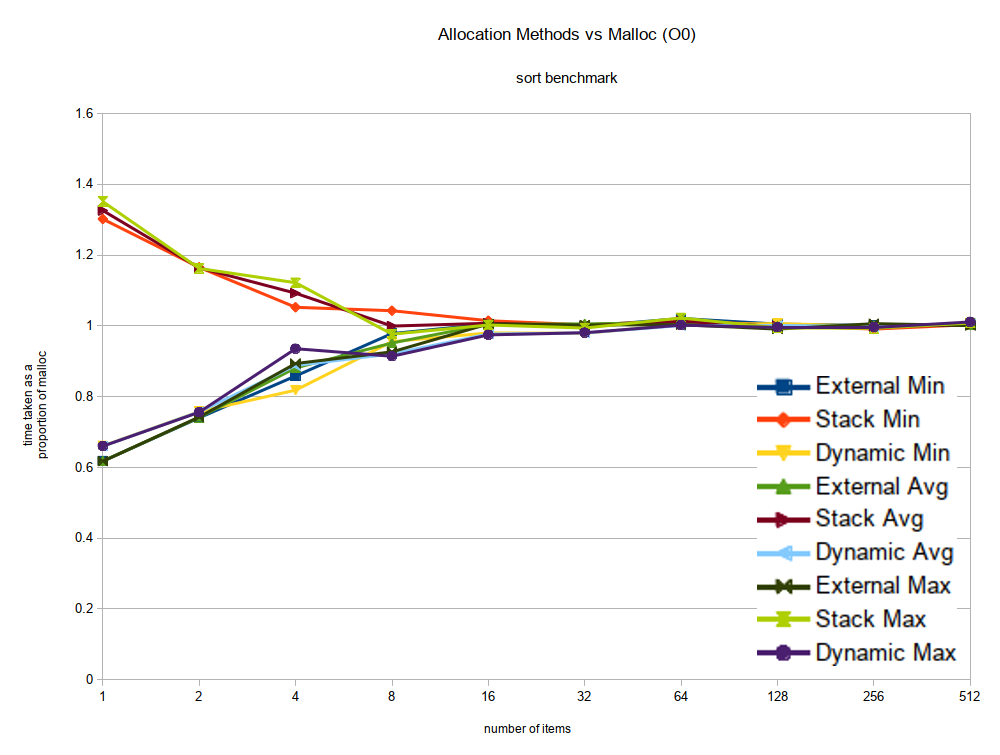
\includegraphics[width=0.8\textwidth]{sort/O0chart}
	\caption{Unexpectedly, \functionname{stack} performs worse than \functionname{malloc}. Others perform as expected. From inspecting the generated assembly, it looks like -O0 produces very inefficient code for alloca.}\label{firstsort}
\end{figure}

\begin{figure}[ph]
	\centering
	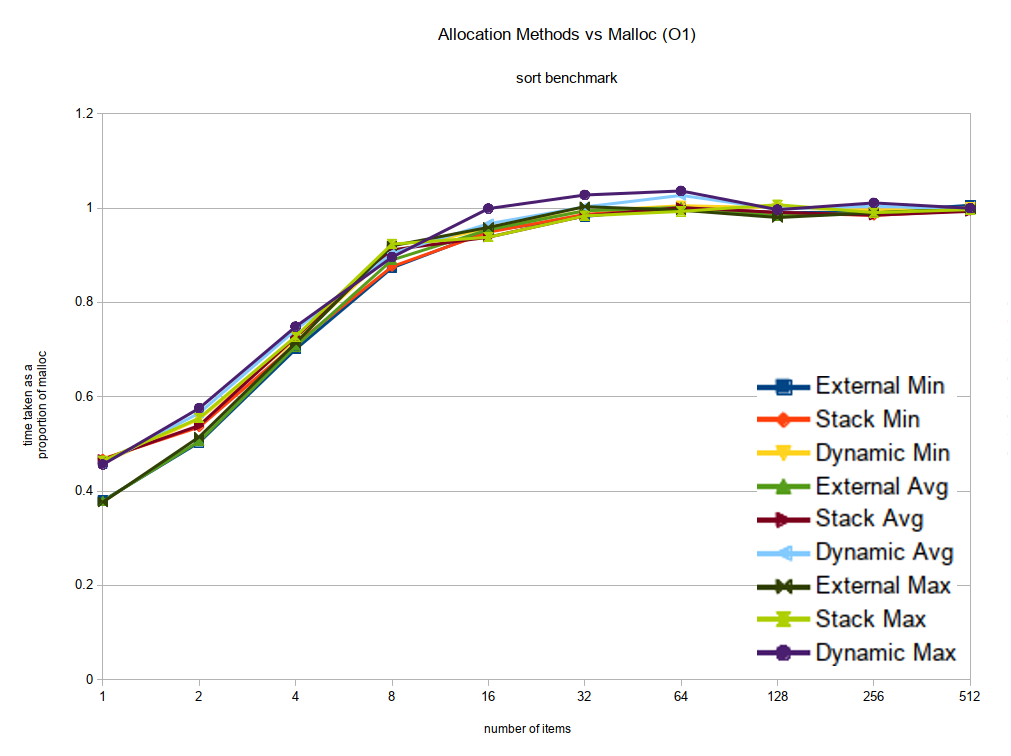
\includegraphics[width=0.8\textwidth]{sort/O1chart}
	\caption{Everything performing mostly as expected. \functionname{stack} and \functionname{dynamic} seem to perform very similarly, with \functionname{dynamic} unexpectedly underperforming \functionname{malloc} before falling back to \functionname{malloc} level performance at around the same input size as the other methods' performance converge with malloc.}
\end{figure}

\begin{figure}[ph]
	\centering
	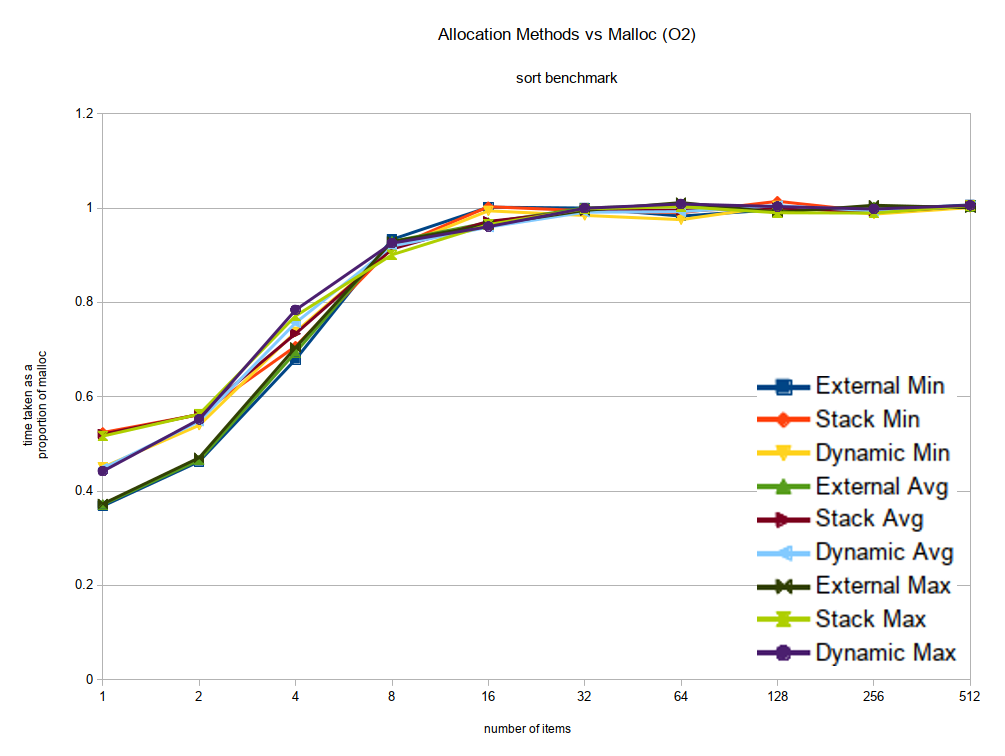
\includegraphics[width=0.8\textwidth]{sort/O2chart}
	\caption{Everything mostly as expected. \functionname{dynamic} shouldn't be faster than \functionname{stack}, but the difference is small and the gap is closed after the first item in any case.}
\end{figure}

\begin{figure}[ph]
	\centering
	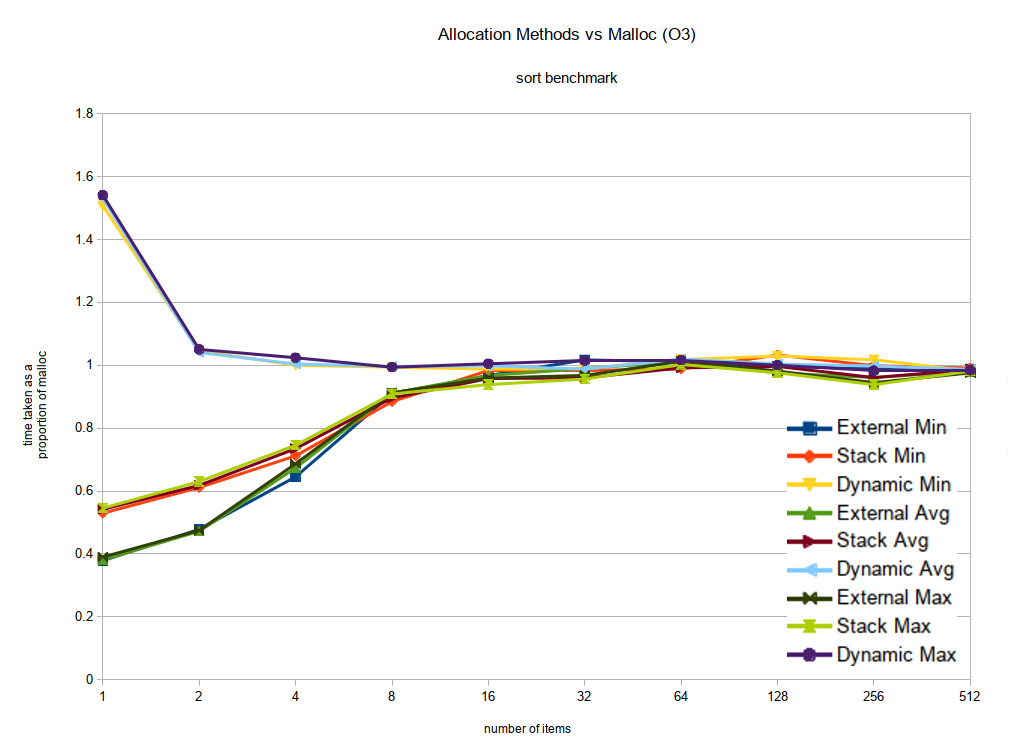
\includegraphics[width=0.8\textwidth]{sort/O3chart}
	\caption{An unusual drop of performance in the \functionname{dynamic} case, with the rest performing as expected. This appears to be caused by function inlining, where the function copying input to the allocated buffer is inlined twice in the \functionname{dynamic} benchmark function. The copy used for the case using \malloc{} is optimised to use \functionname{memcpy} while the other does not. This causes the \functionname{stack} case to perform worse due to the slow copy, rather than any allocation issue.}
\end{figure}

\begin{figure}[ph]
	\centering
	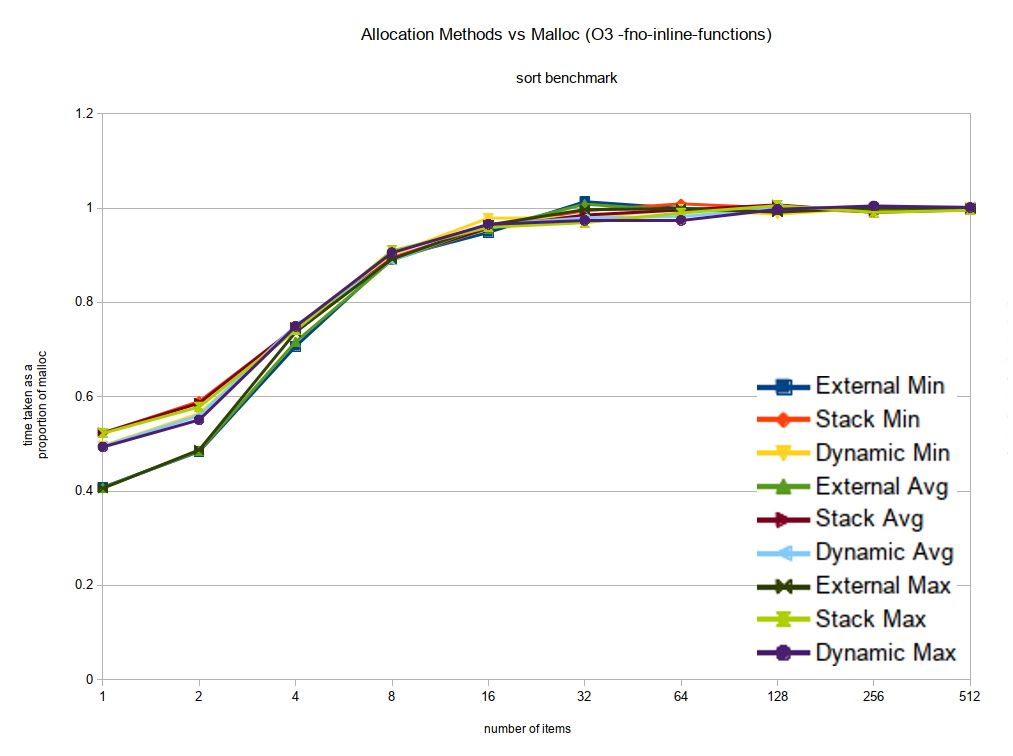
\includegraphics[width=0.8\textwidth]{sort/O3chart-no-inline}
	\caption{The same as the figure above, but with function inlining disabled. Once again, \functionname{dynamic} slightly outperforms \functionname{stack} on small cases.}\label{lastsort}
\end{figure}

\subsection{Comparison to Predictions}

Results largely matched the predictions, with the exception of \functionname{dynamic} outperforming \functionname{stack} narrowly. This may be due to the generated code for \functionname{alloca} being slower than the simple check required by the \functionname{dynamic} case.

These results bode well, especially since the lack of significant performance difference between \functionname{dynamic} and \functionname{stack} means that the safer option, \functionname{dynamic} can be used without issue in real code.

\pagebreak

\section{Specialised Benchmark, Parallel Allocations}

The second benchmark involves a large number of allocations and minimal busy work.

The setup code is identical to the setup for the sort benchmark described above, but instead of calling each function a fixed number of times it sets up a number of threads (in this case 4) which all call the function simultaneously for a total of 2 seconds. This is repeated a number of times (in this case 10) and the number of times the benchmark function was successfully called is taken as an indication of performance.

However, instead of sorting the input data, the functions simply copy the input data to the allocated buffer. The allocation types used are the same as in the sort benchmark.

\subsection{Program Reasoning}

This benchmark seeks to produce a ceiling for performance increases. While there are many implementations of \malloc{}, most involve locks at some level of granularity. In particular, this benchmark was run using glibc's \malloc{}, which does take locks internally~\cite{glibcmalloc}. This benchmark seeks to maximise the contention of these locks, allowing the benchmarking functions to avoid losing time to unavailable mutexes by avoiding \malloc{}s, making them faster by comparison.

\subsection{Predictions}

The predictions are the same as in the sort benchmark, but the speed increases should be more significant.

\subsection{Patch Code}

Refer to the benchmark code in the \texttt{src/parallel} directory in Appendix~\ref{codeappend}.

\subsection{Results}

In the diagrams in Figure~\ref{firstparallel} through Figure~\ref{lastparallel}, the y axis represents the number of function calls completed for a given allocation method compared to the \functionname{malloc} benchmark, while the x axis represents the size of the input data. Values above 1 on the y axis outperform \malloc{}.

The values in the diagrams are taken from a number of runs, from which the top third and bottom third of values were dropped as outliers. The minimum, maximum and mean values were then taken from the remaining values.

\begin{figure}[h]
	\centering
	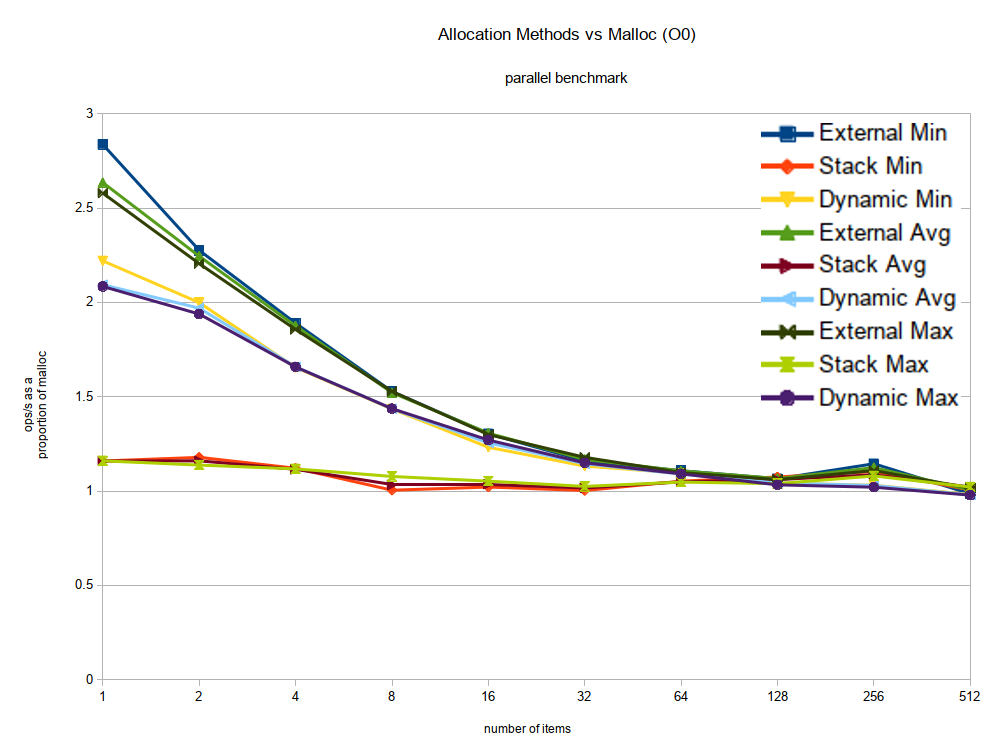
\includegraphics[width=0.8\textwidth]{parallel/O0chart}
	\caption{\functionname{stack} performs poorly again, although this time it still outperforms \functionname{malloc}. Other allocation methods perform as predicted.}\label{firstparallel}
\end{figure}

\begin{figure}[p]
	\centering
	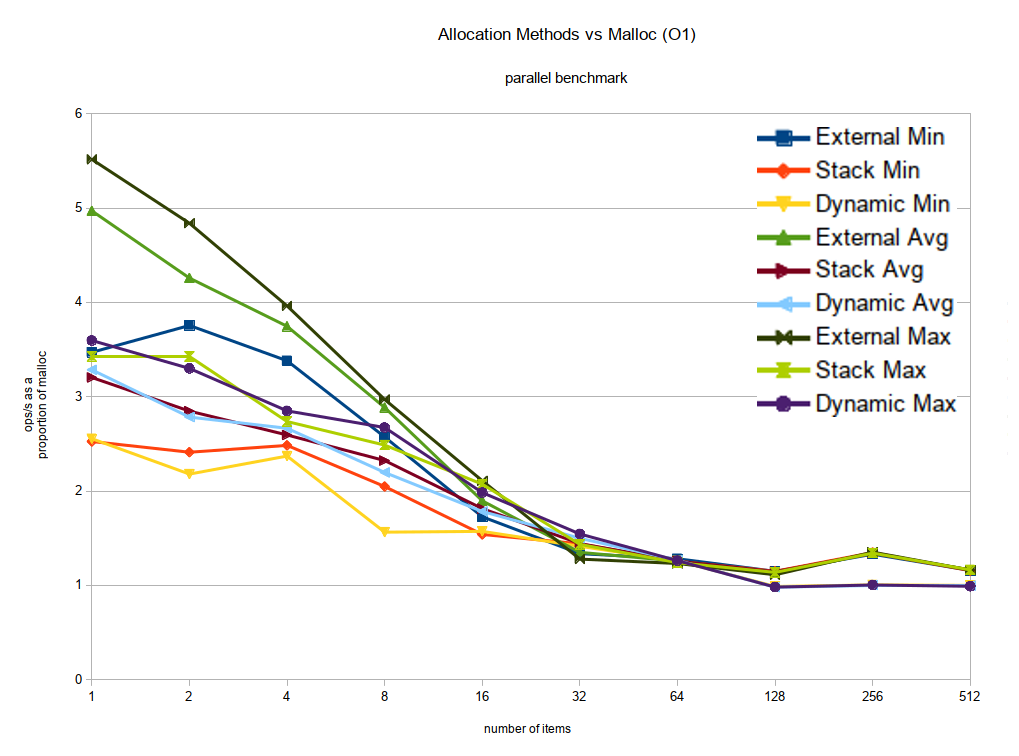
\includegraphics[width=0.8\textwidth]{parallel/O1chart}
	\caption{As seen in the sort benchmark, \functionname{stack} and \functionname{dynamic} perform roughly the same, while external outperforms both. Unlike the sort benchmark, \functionname{stack} and \functionname{external}'s performance benefits don't completely drop off on large input data.}
\end{figure}

\begin{figure}[p]
	\centering
	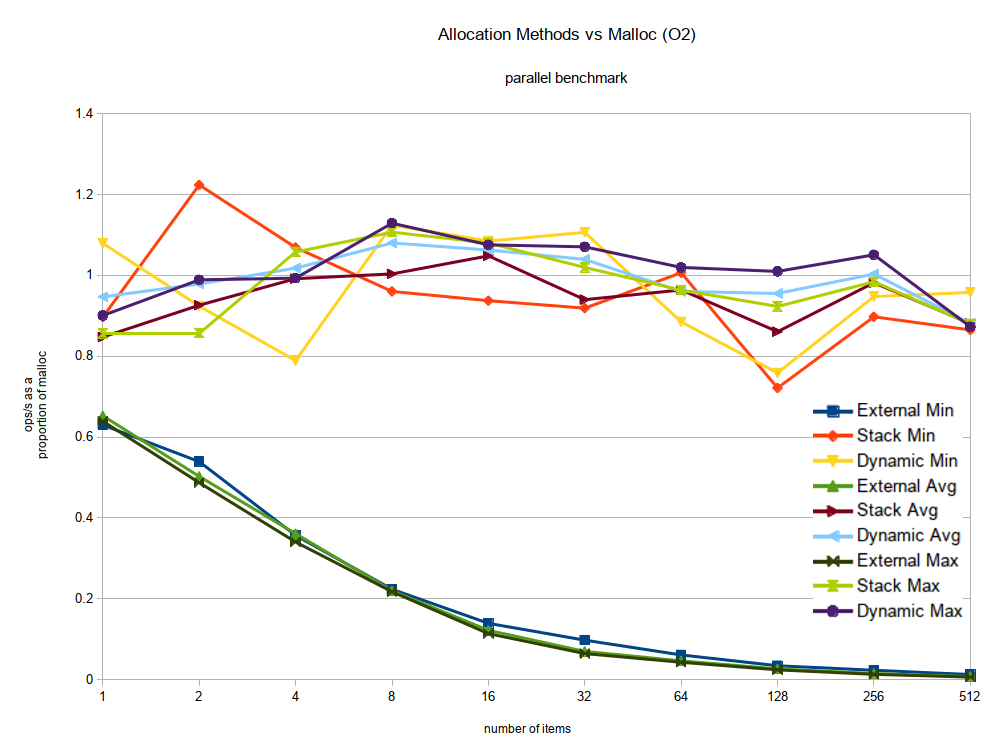
\includegraphics[width=0.8\textwidth]{parallel/O2chart}
	\caption{At this optimisation level the compiler was able to determine that the results of the copying in the benchmark functions were not being used, so the entire functions got optimised out other than the \functionname{external} method, which essentially degenerates to a \functionname{memcpy}. Higher optimisation levels yield the same result.}\label{lastparallel}
\end{figure}

\subsection{Comparison to Predictions}

Similarly to the sort benchmark, results mostly matched the predictions. As expected, performance increases were much more significant than in the sort benchmark. This is expected, as the changes made here are essentially the same as replacing a locking algorithm with a wait-free algorithm.

However, the situations in which this sort of performance increase would be possible are quite limited, as programs are not often allocating at such a high rate.

\pagebreak

\section{Real World Benchmark, \toolname{cURL} Patch}

The third and last benchmark involves a more careful analysis of Stenberg's patch to \toolname{cURL}~\cite{curlmalloc}. It covers both parts of the change described in Section~\ref{backgroundsec}.

The benchmark is performed by cloning \toolname{cURL}'s source and checking out\footnote{A checkout in this context refers to \texttt{git-checkout}, whereby the state of the code is rewound to a given point} the commits in which the changes were made.

In order to test the linked list changes, simply running regular \toolname{cURL} requests is enough, as indicated by the blog post. For the polling function changes, one of the code samples distributed with the \toolname{cURL} source code exercises the exact function to be benchmarked, \functionname{curl\_multi\_wait}.

\subsection{Program Reasoning}

Clearer figures for the performance impact on a real-world program were needed. The two previous benchmarks demonstrate theoretical improvements in carefully constructed scenarios, but to gain a better impression of the real-world impact, real-world code must be tested.

Since the blog post lumps in all changes from some 230 or so commits, it can't be assumed to only be a result of the allocation changes. The goal of this benchmark is to isolate the changes with their effects.

\subsection{Predictions}

Given the results of the previous benchmarks and from the blog post, results are expected to be noticeable in the direction of outperforming \malloc{}, but smaller than described in the blog post.\\
This is accounting for the fact that allocations alone were unlikely to account for 30\% of the execution time as suggested in the blog post. While a large speed-up was shown in the benchmarks, they were designed primarily around allocations and took care to only measure times at the sites where allocations were changed.

By contrast, \toolname{cURL}'s timing cannot focus in only on allocation sites, and if it did focus on only the allocation sites it could miss knock-on effects from the change.

Note that the polling function, \functionname{curl\_multi\_wait}, is benchmarked with 1 and 11 file descriptors. The single file descriptor benchmark is intended to trigger the best case, where a small heap allocation is replaced with a stack allocation, whereas the 11 descriptor benchmark is intended as a control, as its performance should be identical before and after the change. This is due to the fact that only up to 10 descriptors are stack allocated.

There are a number of changes included in the linked list changes, such as: changing initialisation functions from a \malloc{}+\functionname{memset} to a single \functionname{calloc} having the same effect; or a cascading effect from the change to the linked list functions being unable to fail due to a lack of memory resulting in less checks being necessary in code using those functions. These changes could all impact the performance, but should favour the new version of the code performance-wise.\\
To test the linked list changes, a single large and empty file was retrieved from a server running locally.

\subsection{Patch Code}

Refer to the \texttt{replicate.sh} script in the \texttt{src/curl} directory in Appendix~\ref{codeappend}. Running this script on a machine with the required dependencies (refer to the \toolname{cURL} source to determine what dependencies are required to build it) will produce the executables used to benchmark and run the benchmark.

\subsection{Results}

In the diagrams in Figure~\ref{firstcurl} through Figure~\ref{lastcurl}, the y axis represents the run-time of the patched version of \toolname{cURL} as a proportion of the time taken to perform the same task by the parent commit. This is used as a proxy for performance. On the x axis, \functionname{curl-llist} is the result of testing the linked list changes, \functionname{curl-multi-wait-1} is the result of testing the polling function changes with a single file descriptor, \functionname{curl-multi-wait-11} is the control using 11 file descriptors.

The min/avg/max times are as reported by the \toolname{time} utility, and a description of the meaning of user/real/sys is in Table~\ref{timestable}.

\begin{table}
	\centering
	\begin{tabularx}{\linewidth}{>{\hsize=0.6\hsize}X >{\hsize=1.4\hsize}X}
		\toprule
		\textbf{Time Type} & \textbf{Description} \\
		\midrule
		real & Wall clock time elapsed, i.e.\ actual time taken from the program starting to when it exits \\
		user & CPU time spent outside of kernel code \\
		sys & CPU time spent in kernel code \\
		\bottomrule
	\end{tabularx}
	\caption{Description of the meanings of times reported by \toolname{time}}\label{timestable}
\end{table}

The values in the diagrams are taken from a number of runs, from which the top third and bottom third of values were dropped as outliers. The user, real, and sys time values were then taken from the remaining values and their minimum, maximum and mean found.

Values less than 1 outperform the parent commit.

\begin{figure}[h]
	\centering
	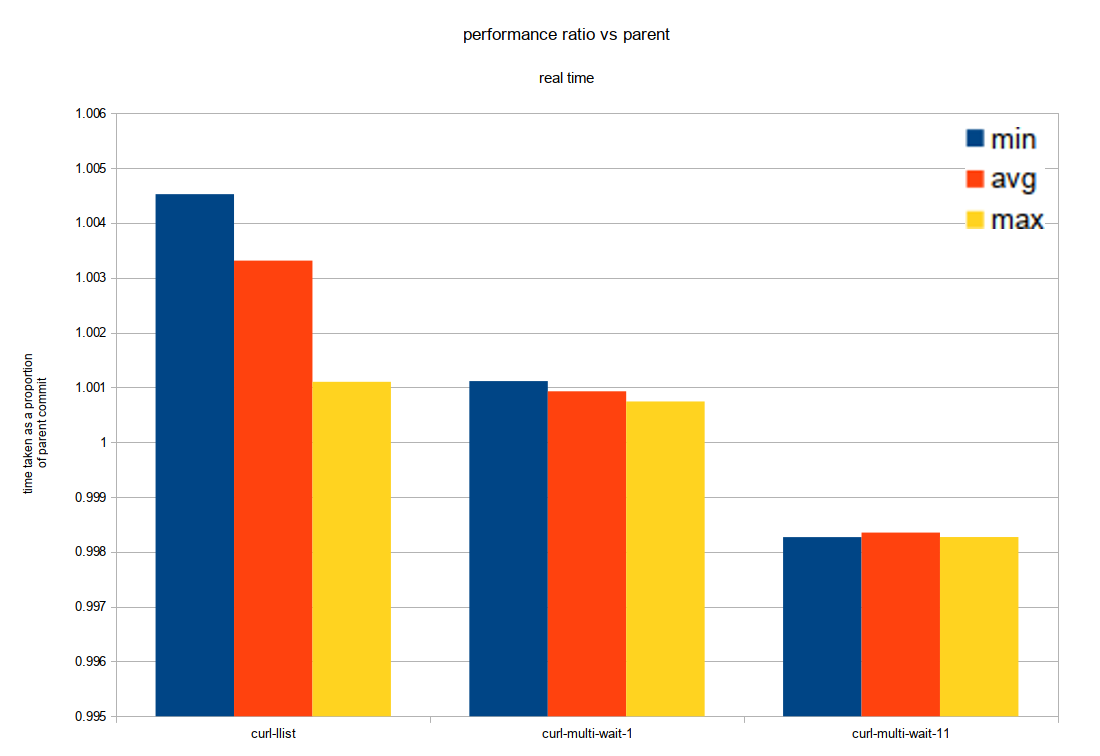
\includegraphics[width=0.8\textwidth]{curl/ratio-real}
	\caption{Nothing varies by more than 0.5\%. The only benchmark that performs better is the one that should perform identically, suggesting that any performance benefit is shadowed by other effects.}\label{firstcurl}
\end{figure}

\begin{figure}[p]
	\centering
	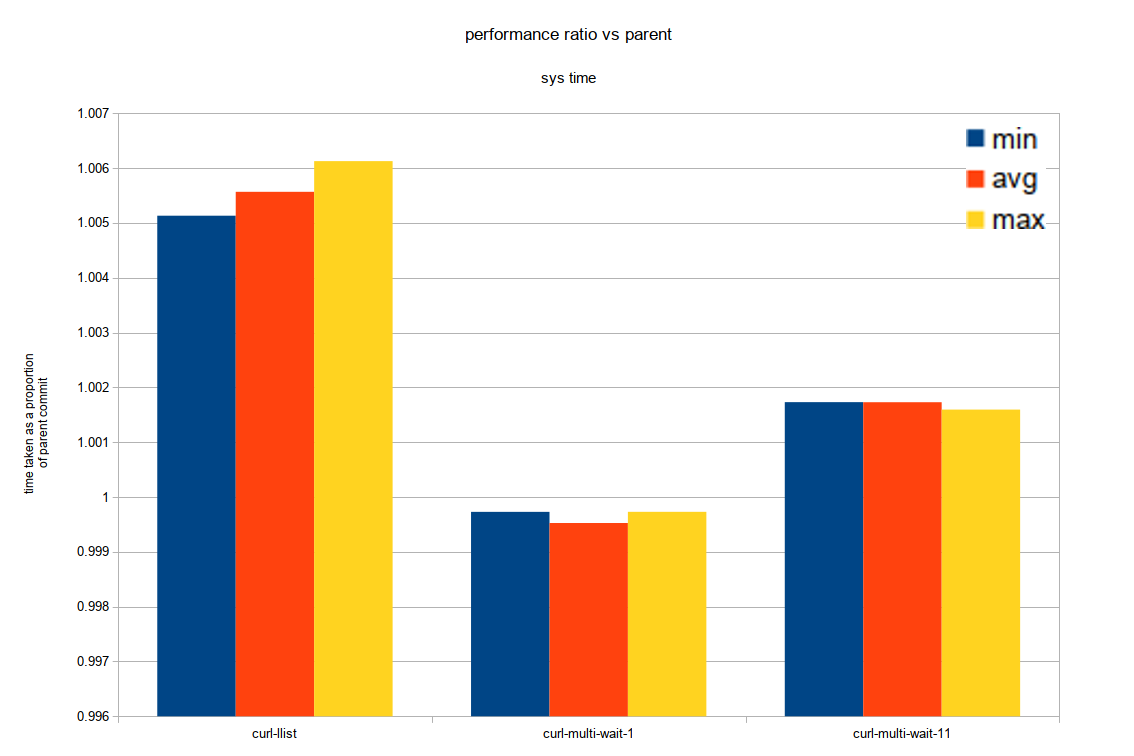
\includegraphics[width=0.8\textwidth]{curl/ratio-sys}
	\caption{sys time should in theory decrease in the first two cases, as less \malloc{}s should mean less time spent in kernel code (such as \functionname{brk}/\functionname{sbrk}/\functionname{mmap}). Once again, the maximum variation is 0.6\%, but in the wrong direction compared to predictions.}
\end{figure}

\begin{figure}[p]
	\centering
	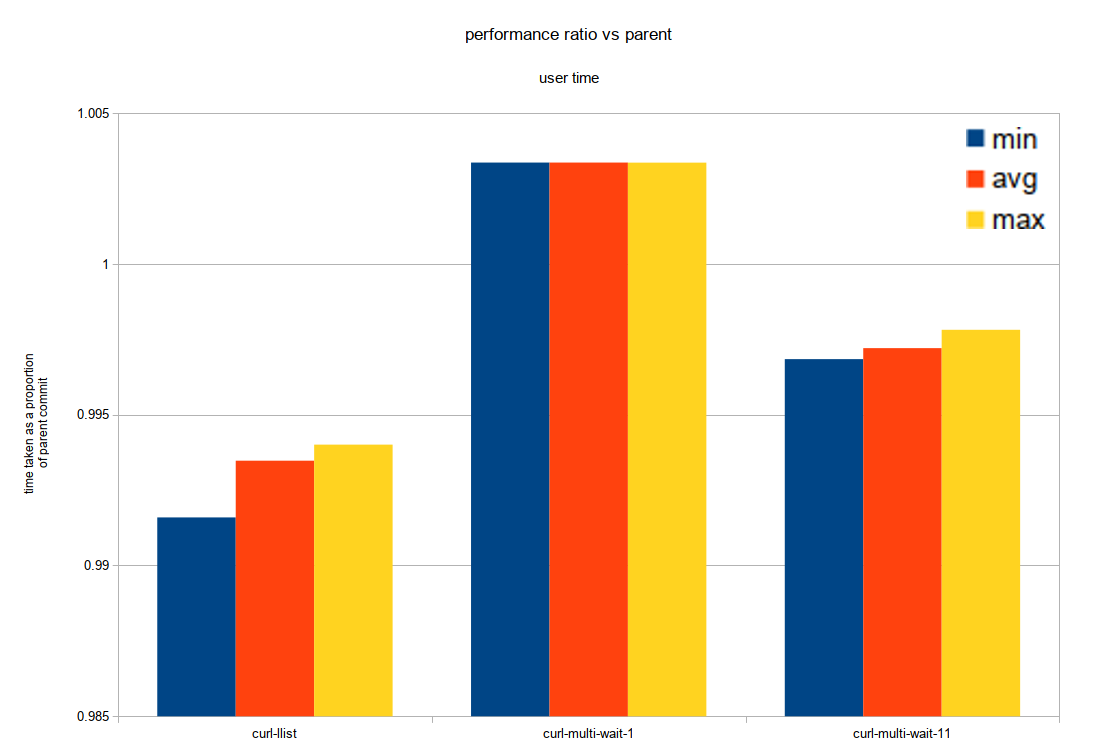
\includegraphics[width=0.8\textwidth]{curl/ratio-user}
	\caption{The llist case should decrease in time thanks to simplified code due to removal of \malloc{}s and use of more efficient library functions (\functionname{calloc} instead of \malloc{} and \functionname{memset}). For the multi-wait case, user time shouldn't really change. This is mostly met, particularly in the llist case.}\label{lastcurl}
\end{figure}

\subsection{Comparison to Predictions}

The results in this benchmark were unexpectedly poor, and differed completely from predictions and indeed from what Stenberg claimed. It seems that one or more of the other commits lumped in with his measurements may have affected the performance difference.


	\chapter{Conclusion}
	\section{Results}

There are two main categories of results to be discussed, the specialised benchmarks and the real world study.

\subsection{Specialised Benchmarks}

The specialised benchmarks, while constructed to be an ideal case for application of the patch, clearly validate that the patch can result in a significant performance increase in specific cases. 

That being said, they also serve as a reminder that even in simple code there may be hidden issues and complexity, such as \functionname{alloca}'s performance at the \texttt{O0} optimisation level in both of the benchmarks, or the unexpected slowdown of the \functionname{dynamic} allocation method at the \texttt{O3} optimisation level in the sort benchmark.

The benchmarks also highlight that, in certain cases, the patch makes no performance difference (little to no difference by 16 items in the sort benchmark, and minimal at the changeover point of 64 items in the parallel benchmark).

Both the \functionname{dynamic} and \functionname{stack} allocation methods as implemented have downsides that are present even when their benefits are no longer being reaped. Note that the following all assume correct usage, for example ensuring that no pointer to the allocated buffer escapes the function scope, or is made accessible to another thread (as threads do not share stacks~\cite{threadstack}).

\subsubsection{\functionname{dynamic} Method Downsides}

The stack frame is bloated with the buffer even when it's not being used, as space must always be allocated for it even if it's determined at run-time that the buffer can't be used.

Depending on where the buffer is declared, whether multiple buffers are declared (if there are multiple inputs that can be copied to stack allocated buffers), and how large the buffers are, locality of the stack could potentially be affected.

The larger stack frames required also increase the likelihood of stack overflow occurring, which will generally result in a segmentation fault due to the invalid access to storage (outside the bounds of the stack)~\cite{c11std}.

\subsubsection{\functionname{stack} Method Downsides}

The most immediate issue with the \functionname{stack} method as implemented is that it unconditionally uses \functionname{alloca} to allocate the buffer. As mentioned before, \functionname{alloca} is not in the C standard and as such is both machine and compiler dependent.

The unconditional allocation also means that the risk of stack overflow, and hence a segmentation fault, is even greater than in the \functionname{dynamic} case, due to use of \functionname{alloca} even if the allocation to be performed is very large.

Another issue with \functionname{alloca} is that it has no way to indicate if the stack frame cannot be extended. Unlike \malloc{}, it never returns \varname{NULL}. This means that is no way to tell if an allocation was successful until the buffer is used, causing a stack overflow and segmentation fault.

\subsubsection{Handling The Downsides}

A better solution than the \functionname{dynamic} or \functionname{stack} allocation methods may be somewhere in between the two. Assuming that the lack of portability of \functionname{alloca} is not an issue, some of its benefits can be used to eliminate some downsides of the \functionname{dynamic} method. This is referred to as the \functionname{hybrid} allocation method hereafter.

Rather than performing a check on the input size and using a statically declared buffer on the stack, the stack allocation itself can be performed with \functionname{alloca} (or, under the C99 standard, a variable length array could be used with portability benefits). This would prevent bloating the stack unnecessarily, allowing only the buffers that will actually get used to be stack allocated.

To handle the increased risk of a segmentation fault, a signal handler could be written capturing the \texttt{SIGSEGV} signal raised. However, signal handlers are extremely restricted in what they can do, which functions they can call, and even which variables they can write to~\cite{signalhandling}. The increase is complexity resulting from needing to write and maintain this signal handler, if a signal handler can even be written to sufficiently generically resolve stack overflow errors\footnote{A trivial, but not necessarily useful, handler simply expands the stack when a stack overflow is detected, but this is unlikely to be possible to do for any extended amount of time, and only works in an environment can be extended at runtime using only functions permissible in signal handlers. This also requires the handler to be able to distinguish between a signal raised due to a stack overflow or due to another reason, such as a \varname{NULL} dereference.}, is unlikely to be justified by any performance benefits gained.

\subsection{Real World Benchmark}

The real world benchmark had disappointing results when compared to the specialised benchmarks, and even to Stenberg's original claims. Results were found to be indistinguishable from variance in the test environment itself, in sharp contrast with the 30\% performance increase claimed~\cite{curlmalloc}.

Despite these results, this doesn't mean that the patch is not worth applying, or at least researching further. Compiler optimisations are known to produce minimal performance benefits individually, instead building up mutually to more significant gains over time and in conjunction with each other.\\
This observation was noted in Proebsting's~Law, in which Proebsting claimed the following, with the figure of doubling every 18 years chosen to match the more well-known Moore's~Law.

\begin{quote}
	These assumptions lead to the conclusion that compiler optimization advances double computing power every 18 years. […] compiler optimizations contribute only 4\% [per year]. Basically, compiler optimization work makes only marginal contributions.~\cite{proebstingdecl}
\end{quote}

These findings were formalised 3 years later by Scott, in which the rate of improvement was estimated to be closer to 2.8–3.6\% per year, or even as high as 4.9\%, depending on what year was taken as the starting point in which compiler optimisations begun to be developed~\cite{proebstingformal}. Scott also notes that there's no reason to give up on compiler optimisations, as any performance benefit is better than none, and in particular there's no reason to turn down existing performance benefits.

\section{State of the Plug-in}

The current state of the \toolname{Forgetful} plug-in is described in Section~\ref{pluginstate}, where the instances of the pattern it can detect are shown and some of its limitations discussed. Some of these limitations are outside of the control of the plug-in, such as the inability to process functions which use recursion, which is imposed by \toolname{EVA}. Other limitations, such as only performing intra-procedural analysis, or the simplified handling of intervals, are internal limitations.

\subsection{Interval Handling}

As mentioned in Section~\ref{alloctrack}, the handling of allocations whose size is some value from an interval is simplistic, with the allocation only being tracked if the entire interval is smaller than the configured maximum allocation size.

As an alternative, intervals could be accepted if some configurable portion of the interval was smaller than the maximum allocation size. This information could then be used in conjunction with profiling data to determine whether the introduction of the \functionname{hybrid} allocation method or similar would be worthwhile.

\subsection{Intra-Procedural Analysis}

\toolname{Forgetful} is currently limited to intra-procedural analysis, due to the additional complexity that inter-procedural analysis would add and the limited time available to complete the project. Tracking the progress of allocated blocks of memory across function boundaries could significantly improve the quality and number of sites that \toolname{Forgetful} can report.

Consider the following code listing:

\lstinputlisting[style=CStyle]{samples/xmalloc.c}

Currently, \toolname{Forgetful} cannot detect that \varname{unreported} is a candidate for replacement, despite \functionname{xmalloc} being a simple wrapper on \malloc{} which cannot return \varname{NULL}. By tracking allocations across function calls, this case could be detected.

This pattern is not unusual, and is similar in structure to a constructor function which allocates and initialises a struct, again being quite a thin wrapper on \malloc{} with some setup steps on the returned value.

Barrett and Zorn defined a term for function invocations which eventually led to a \malloc{}, calling them length-N call chains, where a length-1 call chain is a direct invocation of \malloc{}. While researching the ability to predict lifetimes at allocation sites, they discovered that length-4 call chains were almost always sufficiently long to determine the lifetime of a given allocation~\cite{predictors}. \\
Their methods and goals were different to this project's, and their figures were found experimentally with a limited number of programs 25 years ago, but their findings suggest that analysing longer call-chains would be of worth.

\subsection{Notification Output}

The output displayed in Section~\cite{alloctrack} is real, but is not representative of \toolname{Forgetful}'s output. As analysis is performed on the normalised AST, it may occasionally reference statements that do not exist in the source code itself. Consider the following code listing:

\lstinputlisting[style=CStyle]{samples/transformedOut.c}

The statement on line 2 is rewritten to the following:

\lstinputlisting[style=CStyle]{samples/normalisedOut.c}

This means that when the allocation is reported, it reports the contents of line 4 as the allocation site, which makes it difficult for the user to discern what allocation is being referred to, as can be seen in the following output from the plug-in.

\lstinputlisting[breaklines=true]{samples/transformed_output.txt}

The formatting of this output raises another issue that could be revisited, which is that the output is not easily machine parsable. This could make it less useful in automated pipelines using the tool to detect issues in pull requests, for example.

\section{Benefit of Further Work}

Would further work in this space (not specifically the plug-in) be beneficial? If so, why/what should be done first?


	\chapter{State of the Art}
	This chapter will discuss:

\begin{itemize}
	\itemsep-0.25em
	\item The short-list of static analysis platforms
	\item Other methods to detect the pattern
	\item Research into performance of allocator methods
	\item Validation of the project research space
\end{itemize}

\section{Static Analysis Platforms}

As mentioned before, three options were considered after the remaining platforms were eliminated for appearing to be relatively unmaintained. These options were \toolname{Frama-C}, \toolname{Infer}, and \toolname{clang-analyzer}.

These are discussed in further detail and in retrospect now that the project's requirements and pitfalls are fully known.

\subsection{\toolname{Frama-C}}

While \toolname{Frama-C} was an acceptable choice for its extensibility and availability of introductory guides to plug-in development~\cite{framaplug}, finding assistance/documentation for it was relatively difficult, even for basic functionality of \toolname{EVA}.

Perhaps a better choice would have been to modify/extend a static analysis tool with a more active and modern community (\toolname{Frama-C}'s irregular releases consist of dumps of source code rather than open and incremental development~\cite{framagit}, with the first beta release in March 2008~\cite{framahydrogen}), which likely would've made it easier to dig into the codebase even if it wasn't built as intentionally for extensibility.

\toolname{Frama-C}'s (open source) community is not hugely active, with only a few external plug-ins available~\cite{framapluglist}, and not many plug-ins having been created between its initial release a decade ago and now. In fact, the plug-in list was last updated 5 years ago.

\subsection{\toolname{Infer}}

To the end of finding a large and active community, Facebook's \toolname{Infer} might have been a better choice. By its own description, \textit{Infer checks for null pointer dereferences, memory leaks, coding conventions and unavailable API’s}~[sic], which suggests it may also have been well suited to the project space due to its emphasis on memory issues and tracking memory.

Facebook first open-sourced \toolname{Infer} in June of 2015~\cite{infergit}, at which point it already supported C, Objective-C, C++, Java ($\le$ 1.7) and contained about 100k LoC\footnote{Lines of Code}. Since then, it has averaged 4–6 commits per day (dependending on whether you count weekends, since many of its contributors will be employed specifically to work on it), now has about 300k LoC, and supports Java 8 as well as the original languages.

While it wasn't explicitly designed for modularity like \toolname{Frama-C}, its internal structure for checkers is consistent and logical, which should make the addition of new checkers not prohibitively difficult, even without much guidance~\cite{infercheckers}.

\subsection{\toolname{clang-analyzer}}

\toolname{clang-analyzer}, which \toolname{Infer} depends on, is the only analyser in this list not written in OCaml, instead being in C++ to match the rest of the \toolname{clang} codebase. Among features listed in its documentation are a few memory analysis checkers (null dereference, double free, stack reference escape detection~\cite{clangchecks}) that could prove to be a useful base to build off. Familiarity with C++ (at least compared to a lack of familiarity with OCaml) could also have proven useful in development, reducing delays.

\toolname{clang-analyzer}'s development is much less active than \toolname{Infer}'s, but still more active (or at least more frequently updated) than \toolname{Frama-C}'s. It also has mailing lists and other community communication channels which could have been useful. It's the oldest of the three, started in September 2007~\cite{clangrelease}, but has had a huge amount of development since then (a caveat here: its full development lifecycle is public, from inception to its current state, unlike the other two, which can make it seem more active).

One unique mark against clang-analyser is its heavy emphasis on OS X related features and tutorials/setup instructions revolving around assumptions of the use of Apple hardware and software, which could cause delays in development, as Apple machines were not available for use.

\section{Alternative Detection Methods}

Other than static analysis/compile-time checking, run-time analysis can also be used to surface issues in the code. This profiling has an added benefit that, used properly, it can better reflect performance under real workloads. There are three main ways of achieving this, which are all different levels of the same thing.

\subsection{Custom Wrapper Functions}

The first method involves a custom allocator wrapper function, which is the approach taken by \toolname{cURL}. In this method, calls to memory management functions are intercepted by redefining them to instead use the custom allocators, using a preprocessor directive such as \texttt{\#define malloc(size) curl\_domalloc(size, \_\_LINE\_\_, \_\_FILE\_\_)} to intercept calls and add in debugging information.

Usage of this system can usually be enabled or disabled at compile time by defining or undefining certain symbols, and a detailed implementation can be seen in \toolname{cURL} itself~\cite{curlallocator}.

This method has the obvious downside that the system must be maintained by its users, who usually have goals orthogonal to it. However, it also allows the most fine-grained control of the three methods, and can easily be extended to also track other functions.

\subsection{Provided Wrapper Functions}

When the fine-grained control of intercepting any given function, or adding more things to profile is not needed, wrapper functions can be found already written available online to be compiled along with your existing code.

Similar to the above, these intercept calls to memory management functions, outputting profiling data to a specified log file. One such example is \toolname{malloc\_count}, which can also track stack usage~\cite{malloccount}. Since these projects are more focused on this specific task, they also attempt to meet standards for formatting of the output, which allows the user to use their profiling data with existing graphing tools for memory profiling dumps.

While this method doesn't have the advantage of fine-tuned control of what exact data is dumped nor which functions are intercepted, it also doesn't suffer the disadvantages of maintenance and development of the system. It also benefits over the next method by being faster.

\subsection{Run-time Profiling/Interception}

Without requiring function interception to be included in code at compile time, hooks can be used to intercept calls to any given function. Programs such as \toolname{Valgrind} can use this functionality, for example, to track memory leaks at run-time by tracking all allocated and freed memory, or determine when uninitialised data is used as if it were initialised (as a branch condition, for example)~\cite{valgrind}.

Similarly, programs such as \toolname{Heaptrack} use hooks\footnote{A hook allows interception of events by either intercepting calls at run-time or rewriting calls before a binary is executed} in order to profile memory usage~\cite{heaptrack}. As such, it requires no changes to the actual source or files included for compilation. However, in order to get more detailed information about allocations (such as the line in the source where it occurs), debug symbols must be included in the binary, which involves the addition of a flag to the compilation command.

As has been the trend in this section, the increased convenience comes with a decrease in tunability. However, again it comes with an improvement in ease of consumption of data, for example \toolname{Heaptrack} is a two part tool, one producing a detailed dump while the other consumes the dump to produce a large number of statistics and graphics.

\section{Performance of Allocator Methods}

This section is concerned with research into the performance of existing allocator methods, and also with potential side-effects resulting from the replacement of a heap allocation with a stack allocation.

\subsection{Locality Impact}

One of the potential side-effects is impact on locality of the data. Replacing dynamic allocations with stack allocation could affect cache-hit frequency, as the stack is likely to be in cache, whereas the next section of the heap may not be, especially if the heap is sectioned out based on allocation sizes. However, Appel and Shao found the effect of using stack or heap allocation for frame allocation to be too trivial to matter in terms of effect on the cache miss rate~\cite{stackvheap}. This suggests that a similar principle may apply to general use of the stack and heap.

They do note that the cache write-miss rate is very high for heap-allocated frames, but this can be mitigated with an appropriate write-miss strategy.

In short, it seems unlikely that the cache miss/hit rate will have a significant impact on the results of the optimisation, but of course architectures and timings have changed over the past two decades and so what was trivial then may not be any more (as cache increases in relative speed).

\subsection{Real-Time Considerations}

Another consideration for the utility of the patch are the different potential target users. For systems with real-time considerations, using stack allocation instead of heap allocation can be beneficial even without improvement in average case performance, due to capping the worst-case performance.

Puaut finds that ratio of average to worst-case performance (obtained analytically) of memory allocation algorithms varies from about 10–10000 (the lower bound algorithms have an average case of about 10x those of the higher bound), while stack allocation has fixed performance, even if bounds checking is added~\cite{mallocperf}. Of course, similar benefits could be obtained with correct use of an allocator designed for that purpose.

However, Puaut also finds that the actual observed ratio of average to worst-case performance ranges from about 1–35, so for real workloads the effect may, again, not be great.

\section{Validation of Project Space}

In order to validate the project space, other attempts to target the same inefficiencies were searched for. Small amounts of short-lived memory is the purview of the youngest generation of generational garbage collection, while other approaches to tackling the same issue could instead go directly to the allocator method in order to explicitly split out these allocations ahead of time.

\subsection{Generation Garbage Collection}

Generational (or ephemeral) garbage collection relies on a hypothesis, supported by empirical measurements, that the most recently created objects are also those most likely to become unreachable quickly.

Supporting this hypothesis, Wilson claims that, while figures vary depending on the source language and program, 80–98\% of all newly-allocated objects ``die within a few million instructions, or before another megabyte has been allocated; the majority of objects die even more quickly, within tens of kilobytes of allocation''~\cite{uniprocessorgc}.

In terms of efficiency, Appel makes the counter-intuitive claim that garbage collection collection can be faster than even stack allocation~\cite{stackvgc}. The claim relies on the usage of a copying garbage collector and a sufficiently large amount of physical memory being made available. Key to the assertion is that not every allocation will need to be handled once it's unreachable, as only objects that survive until the next garbage collection need to be handled by copying them to the new heap.

Exact formulae are provided in the paper, parametrisable in terms of: the memory available; instructions taken to copy an object; average size of an object; instructions taken to explicitly free an item; number of allocated items; and instructions taken to traverse the object graph. However, the conclusion is that even arbitrarily efficient explicit freeing always eventually lose out in performance to a garbage-collected system with larger amounts of available memory.

\subsection{Allocator Replacement}

There are cases where garbage collection can't be used for one reason or another (insufficient timing guarantees for real-time systems for example), so in these cases alternate systems can be used to take advantage of the large proportion of short-lived allocations.

Barrett and Zorn discus the use of profiling to determine which allocations are short-lived. In particular, they describe an algorithm for lifetime prediction using a combination of profiling data, allocation site and allocation size which (depending on which program they used to benchmark) correctly predicted the lifetimes of 42–99\% of allocations. Clearly these results vary too widely (and only 4 programs were benchmarked) to be a definitive indicator of whether this method is worthwhile~\cite{predictors}.

However, in the same paper, simulated results using lifetime prediction to segregate allocations into specialised areas in the heap (with shorter-lived allocations/deallocations being cheaper) showed that there was significant potential for reduction of memory overhead, improvement of reference locality (by having recent allocations in a small section of the heap likely to be in cache) and occasionally improvement of performance. This system bears some resemblance to concepts in generational garbage collection.


	\chapter{Future Work}
	\epigraph{A program is never less than 90\% complete, and never more than 95\% complete.}{Terry Baker}

Any non-trivial work is never complete, and the optimisation field in particular is provably endlessly expandable due to the \textit{full employment for compiler writers} theorem~\cite{compilerimpl}. To the end of inspiring such work, listed below are some ideas for potential improvements on the \toolname{Forgetful} plug-in and in the general space of compiler optimisations.

\section{Further Work on Allocation Changes}

This section discusses potential further work directly on the \toolname{Forgetful} plug-in, and also in the general area of memory allocation research.

\subsection{Detecting Arbitrary Memory Allocations}

The current implementation only finds allocations based on uses of \malloc{} and \free{}. Other ways to allocate memory exist (\functionname{calloc}, \functionname{realloc}, direct uses of \functionname{mmap} and \functionname{sbrk}), and platforms that stand to gain the most from this optimisation may have their own implementations.

An extension to this work could involve allowing an arbitrary list of functions declared to allocate or deallocate memory, but this would require the existence of annotated files specifying their behaviour so that \toolname{Frama-C} can be used to its full potential (particularly for value analysis, which relies on these specifications).

Alternatively, the depth of analysis could be extended to attempt to automatically determine which functions might allocate memory. Assuming a UNIX-like platform, searching for \functionname{mmap} or \functionname{sbrk} calls would allow the detection of those functions.\\
The approach propagating allocation information already exists, in some form, in the \toolname{Infer}~\cite{fbinfer} static analyser, so future work could also involve extending that platform instead.

\subsection{Automatically Performing Fixes}

Ideally, fixes would be automatically generated and patched into the code as a pre-compilation step, avoiding added complexity from the programmer's point of view while still taking advantage of performance and memory benefits.

Potential intermediate steps toward that goal could involve generation of patches that could be manually applied to code before compilation, introducing the optimisation.

Based on the documentation for \toolname{Frama-C} and one of its plug-ins, \toolname{PathCrawler}, it is unclear whether there are code generation capabilities in \toolname{Frama-C} or if the plug-in introduced them itself. If this capability is not present, this goal may be very complicated to complete, and potentially not worthwhile.

\subsection{Higher Precision in Allocation Sizing Calculations}

\toolname{Frama-C} has built in defaults for sizes of various types, which mostly seem to be based on a 32-bit architecture. As a result, size calculations can be inaccurate, for example on 64-bit machines where factor of 2 inaccuracies will occur in any size calculation involving pointers.

Not accounting for these differences will lead to \toolname{Forgetful} recommending replacements at sites where, in practice, more memory than the configured maximum is allocated. \toolname{Frama-C} provides a system to define sizes of all the types, which could be exposed to users, allowing them to specify their architecture details.

\subsection{Alternative Architectures}

For the sake of practicality and the limited time available to source and configure machines on other architectures, the analysis presented was only performed on a single x86 machine. To be certain whether these results apply more generally, the analysis should also be performed on other architectures.

\section{General Compiler Optimisation Research}

This section is concerned with the more general area of research into compiler optimisations, both in terms of optimisations to be researched or implemented, and also in terms of research into measurement of optimisations.

\subsection{Potential For Bias Against Optimisations In Evaluation of Proebsting's Law}

In his research into Proebsting's law, Scott notes four potential issues with his analysis~\cite{proebstingformal}. While he suitably discusses and dismisses the first three, the fourth is briefly covered and then assumed to not disproportionately affect the analysis. This fourth issue is that it is impossible to fully disable all optimisations in a compiler through configuration.

The method used involves compiling certain benchmarks first with all compiler optimisations disabled through configuration options, then again with the flags recommended by the vendors for those benchmarks. The assumptions are that a compiler with all optimisations disabled is equivalent to a compiler before new optimisations were discovered and implemented. However, certain optimisations such as peephole optimisations or more efficient code generation techniques cannot be disabled. This results in a baseline program which is more efficient than it would have been, had it been compiled with an older compiler~\cite{proebstingformal}.

As a result of a more efficient baseline program, the relative improvement is lower, biasing the results against higher performance increases.

Further work determining a more accurate and general figure (or figures) for year-on-year improvements that can be reasonably expected of compiler optimisations would provide a point of reference to determine whether a given optimisation is worth introducing to industrial compilers.

\subsection{Disproportionate Improvement of Optimisations}

Proebsting's Law seeks to make a general prediction about performance improvements due to compiler optimisations over time but, as Scott notes, different types of benchmarks display very different levels of performance increase.

It is noted that floating point benchmarks improved significantly more than integer based benchmarks, which means that optimisations have disproportionately benefited scientific applications~\cite{proebstingformal}.

Similar to the previous section's suggestion to produce figures to compare to, perhaps determining expected figures for various areas of research or classes of program could also be worthwhile.

\subsection{Targets for Optimisation}

Contrary to the usual definition, \textit{target} here does not refer to a target machine or architecture, but instead the goal of a given optimisation and the research into it.

In declaring his law, Proebsting also suggests that future research be directed at improving programmer productivity, rather than micro-optimisations~\cite{proebstingdecl}. Pugh suggests the same, and that higher level constructs and designs have more space for improvement than expression and statement-level optimisations~\cite{optimisationrelevant}.

Alongside these suggestions, Pugh lists a number of areas in which research may be worthwhile, including the following:

\begin{itemize}
	\itemsep-0.25em
	\item Making higher level constructs and data types as efficient as primitives, with little to no programmer intervention
	\item Optimising safety checks away, so that safe code can be as performant as unsafe alternatives
	\item Performing optimisations that allow clean and easily readable code to be as efficient as carefully hand optimised code using techniques such as loop unrolling and cache-aligning related data (this is already performed to some degree in industrial compilers, but can require programmer intervention and cluttering code to maximise performance~\cite{gccloops})
	\item Allowing language level guarantees about certain optimisations and performance, such as guaranteeing that tail-call elimination will occur (this specific case is tentatively offered by Haskell~\cite{haskelltail})
	\item Replacing inefficient algorithms with efficient versions having the same results, such as detecting presence of a quadratic stable sort and replacing it with a linearithmic stable sort
	\item Providing stronger safety guarantees for concurrent programs
\end{itemize}

\subsection{Benchmark Design}

Benchmarks are often designed, as the specialised ones in this project were, to elicit certain behaviours. As such, they are carefully tailored, hand optimised, and written at a very low level to avoid other behaviours that may affect their performance. However, this means that these benchmarks do not reflect real world code, and Pugh even argues that their style is so poor and unrealistic that they shouldn't be exposed to undergraduates~\cite{optimisationrelevant}.

Instead, he suggests, they should be written to reflect that real code is complex, and should use techniques and utilities such as higher level constructs, parallelism and more modular components. This would enable benchmarking of bigger picture optimisations that the preceding sections' work would support.


	\clearpage
	\addcontentsline{toc}{chapter}{Bibliography}
	\printbibliography
\end{document}
